% Copyright 2026 Sreeram Anil
% SPDX-License-Identifier: CC-BY-4.0
% =============================================================================
%  Hybrid neural-network / extended Kalman filter (NN-EKF)
% =============================================================================
\chapter{Hybrid neural residual EKF (NN-EKF)}
\label{ch:nnekf}

\section*{At a glance}
\begin{tabular}{@{}l>{\raggedright\arraybackslash}p{0.76\textwidth}@{}}
Family & learning (data-driven) \\
Header & \texttt{include/estkit/learning/nn\_ekf.hpp} (model), \texttt{mlp.hpp} (network) \\
Registered name & \texttt{NN-EKF} \\
State dimension & $n_x = 4$ (cell model) --- the EKF itself is generic in $n_x,n_u,n_y$ \\
Cost per step & EKF $\mathcal{O}(n_x^3)$ $+$ three $3\!-\!10\!-\!1$ forward passes
($\num{120}$ MAC, $30$ \texttt{tanh}) \\
Memory & filter \SI{4.3}{\kilo\byte} (OCV table included) $+$ \SI{0.5}{\kilo\byte} weights \\
Primary references & \cite{charkhgard2010nnekf,hornik1989,plett2004ekf3,kingma2015adam} \\
\end{tabular}

\section{Motivation and aerospace/BMS relevance}
Chapter~\ref{ch:nndirect} showed what a purely data-driven regressor costs: it throws away a
century of circuit theory and buys extrapolation risk in return.  The opposite extreme --- the
plain EKF --- keeps all of the physics and is limited by exactly the physics it does not have.
Two of this benchmark's scenarios expose that limit directly.  On \texttt{preisach} the truth cell
carries a distributed Preisach hysteresis operator \citep{mayergoyz1991hysteresis,
baronti2014hysteresis} spanning $\pm\SI{15}{\milli\volt}$, while the estimator model has the
one-state Plett hysteresis of magnitude $M = \SI{5}{\milli\volt}$; the model simply cannot produce
the missing $\SI{10}{\milli\volt}$, so the SOC estimate absorbs it and the EKF settles at
$\mathrm{rmse_{ss}} = \SI{0.20}{\percent}$ --- four times its \SI{0.05}{\percent} on the nominal
cell.  On \texttt{aged\_cell} the truth cell has lost \SI{15}{\percent} of its capacity and grown
its series resistance by \SI{37.5}{\percent}, and the EKF settles at \SI{1.52}{\percent}.  Neither
is a tuning problem; both are structural model errors.

\citet{charkhgard2010nnekf} proposed the natural compromise: keep the equivalent-circuit model and
the Kalman recursion, and let a small neural network supply the part of the output equation the
circuit cannot express.  The physics still carries the state dynamics --- the Coulomb-counting
integrator, the RC relaxation, the temperature scheduling --- so the estimator keeps its
covariance, its innovation sequence and its ability to extrapolate along the model.  The network
is confined to a bounded, saturated correction of a \emph{single scalar}, the predicted terminal
voltage.  From a certification standpoint this is a very different proposition from
Chapter~\ref{ch:nndirect}: the learned item has a bounded output ($\pm\SI{60}{\milli\volt}$ by
construction), a bounded influence on the state (through the Kalman gain), and a fallback that is
a fully specified filter (set the trust factor $g$ to zero and the estimator becomes the plain EKF,
bit for bit).

The price, which this chapter measures rather than hides, is that the residual model is only valid
for the cell \emph{population} it was fitted to.  Applied to a specimen from a different
population, it injects a systematic voltage error that the filter dutifully converts into an SOC
bias.

\section{Problem statement and assumptions}
The estimator model is the discrete-time 2-RC ESC model of Chapter~\ref{ch:ecm},
\begin{equation}\label{eq:nne-model}
\vx = [\soc, v_1, v_2, h]^\T,\qquad \vu = [i, T]^\T,\qquad
h_{\mathrm{ECM}}(\vx,\vu) = \ocv(\soc,T) + M h - v_1 - v_2 - R_0(T)\, i .
\end{equation}
Write $y_k$ for the measured terminal voltage.  The method assumes:

\begin{assumption}[Separable output error]\label{as:nne-sep}
The mismatch between the true and modelled output can be written, to the accuracy required, as a
static function of $(\soc, i, T)$:
$y_k = h_{\mathrm{ECM}}(\vx_k,\vu_k) + r(\soc_k, i_k, T_k) + \vv_k$, with $\vv_k$ zero-mean.
\end{assumption}

\begin{assumption}[Correct dynamics]\label{as:nne-dyn}
The state equation $\vx_{k+1} = f(\vx_k,\vu_k)$ is correct up to the process noise; the network
corrects the output equation only.
\end{assumption}

Assumption~\ref{as:nne-sep} is exactly right for a thermodynamic or ohmic mismatch (an entropic
term, a wrong $R_0$) and only approximately right for hysteresis, which depends on the SOC
\emph{history} and not on the instantaneous SOC.  It becomes a good approximation on this
benchmark because all three missions are essentially monotone discharges from $z_0 = 0.95$: along a
single discharge branch the Preisach output \emph{is} a function of $\soc$.  Section~\ref{sec:nne-res}
returns to the consequences of that qualification.

\section{Derivation}

\subsection{The augmented output equation}
Define the residual network $r:\real^3\to\real$ and augment \cref{eq:nne-model} by
\begin{equation}\label{eq:nne-h}
h(\vx,\vu) \;=\; h_{\mathrm{ECM}}(\vx,\vu) \;+\;
\operatorname{sat}_{r_{\max}}\!\bigl(g\, r(\soc, i, T;\theta)\bigr),
\end{equation}
where $g\in[0,1]$ is a trust factor (default $1$), $r_{\max} = \SI{60}{\milli\volt}$ and
$\operatorname{sat}_{a}(x) = \max(-a,\min(a,x))$.  The saturation is a safety element, not a
modelling one: it bounds what a badly extrapolating network can do to the filter, in the same
spirit as the output limiter that would be placed around any learned item in an airborne system.
$r$ is the one-hidden-layer \texttt{tanh} network of Chapter~\ref{ch:nndirect}, here with
$n_\phi = 3$, $n_h = 10$, $n_{\text{out}} = 1$ --- $\num{51}$ parameters.  It is deliberately tiny:
the residual is a smooth, low-dimensional surface, and a larger network would fit the
\SI{2}{\milli\volt} sensor noise of the training data.

Because \cref{eq:nne-h} leaves the state equation untouched, the augmented model still satisfies
the estkit model concept and the ordinary EKF of Chapter~\ref{ch:ekf} is used \emph{unchanged}.
Only the measurement Jacobian picks up the network sensitivity:
\begin{equation}\label{eq:nne-H}
\mH(\vx,\vu) = \mH_{\mathrm{ECM}}(\vx,\vu) +
\Bigl[\ \tfrac{\partial r}{\partial \soc},\ 0,\ 0,\ 0\ \Bigr],
\qquad
\mH_{\mathrm{ECM}} = \Bigl[\ \tfrac{\partial\ocv}{\partial\soc},\ -1,\ -1,\ M\ \Bigr].
\end{equation}
The network derivative is taken by central differences,
\begin{equation}\label{eq:nne-fd}
\frac{\partial r}{\partial \soc}\Big|_{\soc} \approx
\frac{r(\soc+\delta,i,T) - r(\soc-\delta,i,T)}{2\delta},\qquad \delta = \num{e-4},
\end{equation}
which for a smooth $r$ has truncation error $\mathcal{O}(\delta^2)\sim\num{e-8}$ and cancellation
error $\mathcal{O}(\epsilon_{\text{mach}}/\delta)\sim\num{e-12}$ in double precision --- far below
any modelling error.  The analytic derivative is available (it is one more backward pass) but two
extra forward passes cost less than the branch-free backward pass and keep the model header
independent of the training code.

\subsection{Measurement-noise inflation}
A residual model fitted to a \emph{population} of cells has a non-zero prediction error on any
individual specimen.  Treating $r$ as exact would make the filter overconfident, so the
measurement-noise covariance is inflated by the residual model's own variance:
\begin{equation}\label{eq:nne-R}
\mR(\vx,\vu) = \underbrace{\sigma_v^2 + \bigl(R_0(T)\sigma_i\bigr)^2}_{\text{sensor}}
\;+\; \sigma_{\mathrm{nn}}^2,
\qquad \sigma_{\mathrm{nn}} = \SI{4}{\milli\volt},
\end{equation}
which is the root-mean-square residual the network leaves on held-out training missions.  This is
the standard treatment of a model-error term as an additional, independent measurement noise
\citep{jazwinski1970}; it is what keeps the filter's innovation sequence consistent and its
$\pm2\sigma$ band meaningful.

\subsection{Fitting the residual}
\label{sec:nne-res}
The training target is the mismatch between the measured terminal voltage and the \emph{nominal}
model evaluated at the true SOC.  For each training mission the nominal ECM is propagated
open-loop from the measured current while the SOC channel is pinned to the ground truth:
\begin{align}
\tilde\vx_k &= [\,z^{\text{true}}_k,\ v_{1,k},\ v_{2,k},\ h_k\,]^\T, &
[v_{1,k+1}, v_{2,k+1}, h_{k+1}] &\text{ from } f(\tilde\vx_k, \vu_k), \label{eq:nne-prop}\\
r^{(k)} &= y_k - h_{\mathrm{ECM}}(\tilde\vx_k, \vu_k), &
\phi^{(k)} &= [\, z^{\text{true}}_k,\ i^{\text{meas}}_k,\ T^{\text{meas}}_k - T_0\,]^\T.
\label{eq:nne-target}
\end{align}
Pinning the SOC is what makes \cref{eq:nne-target} a \emph{model-error} residual rather than an
\emph{estimation}-error residual: it is the voltage the correct-SOC nominal model fails to explain,
which is precisely the quantity \cref{eq:nne-h} has to supply.  The RC states and the hysteresis
state are propagated open-loop, so their own (small) mismatch is part of the target as well.  The
loss, optimiser, standardisation, initialisation and learning-rate schedule are identical to
Chapter~\ref{ch:nndirect}, \crefrange{eq:nnd-loss}{eq:nnd-lr}, with $E = 12$ epochs.

\section{Algorithm}
\begin{algorithm}[H]
\caption{NN-EKF --- one sampling period (offline fit as in Chapter~\ref{ch:nndirect})}
\begin{algorithmic}[1]
\Require $\xplus_{k-1}, \Pplus_{k-1}, \vu_{k-1}, y_k, \vu_k$; frozen network $\theta$; $g$, $r_{\max}$
\Statex \textbf{Time update} (unchanged from the EKF; the network does not enter $f$)
\State $\mF \gets \partial f/\partial\vx|_{\xplus_{k-1},\vu_{k-1}}$
\State $\xminus_k \gets f(\xplus_{k-1},\vu_{k-1})$
\State $\Pminus_k \gets \mF\,\Pplus_{k-1}\mF^\T + \mQ(\xminus_k,\vu_{k-1})$
\Statex \textbf{Residual evaluation}
\State $\rho \gets \operatorname{sat}_{r_{\max}}\!\bigl(g\,r(\xminus_{k,1}, u_{k,1}, u_{k,2})\bigr)$ \Comment{$\num{120}$ MAC, $10$ \texttt{tanh}}
\State $\partial\rho/\partial \soc \gets$ central difference \cref{eq:nne-fd} \Comment{two more forward passes}
\Statex \textbf{Measurement update}
\State $\mH \gets \mH_{\mathrm{ECM}}(\xminus_k,\vu_k) + [\,\partial\rho/\partial\soc,0,0,0\,]$
\State $\mR \gets$ \cref{eq:nne-R};\quad $\mS \gets \mH\Pminus_k\mH^\T + \mR$;\quad
       $\mK \gets \Pminus_k \mH^\T \mS^{-1}$
\State $\nu \gets y_k - \bigl(h_{\mathrm{ECM}}(\xminus_k,\vu_k) + \rho\bigr)$
\State $\xplus_k \gets \xminus_k + \mK\nu$
\State $\Pplus_k \gets (\mI-\mK\mH)\Pminus_k(\mI-\mK\mH)^\T + \mK\mR\mK^\T$ \Comment{Joseph form}
\State $\xplus_k \gets \operatorname{constrain}(\xplus_k)$ \Comment{$\soc\in[-0.05,1.05]$, $h\in[-1,1]$}
\Ensure $\xplus_k, \Pplus_k$
\end{algorithmic}
\end{algorithm}

\section{Application to the battery model}
The augmented model is realised as \texttt{NnEcmModel}, a thin wrapper that owns an
\texttt{EcmModel}, a pointer to the shared trained network, and the three tuning constants
$g$ (\texttt{r\_gain}), $r_{\max}$ (\texttt{r\_max}) and $\sigma_{\mathrm{nn}}$
(\texttt{sigma\_nn}).  It forwards $f$, $\mF$, $\mB$, $\mQ$ and \texttt{constrain} to the base
model and overrides only $h$, $\mH$ and $\mR$; the registered estimator is therefore literally
\texttt{Ekf<NnEcmModel>}.  A default-constructed \texttt{NnEcmModel} holds a null network pointer
and is bit-for-bit the plain ECM, which is both the safe fallback and the reason the one-off
training is not triggered at program start-up: the network is bound only by the
\texttt{EstimatorConfig} constructor, i.e.\ inside \texttt{CellEstimator::reset()}.

\paragraph{Training set.}  Missions \texttt{fixed\_wing} and \texttt{hover\_hold} (never
\texttt{evtol}), scenarios \texttt{nominal}, \texttt{cold} and \texttt{hot} so that the
temperature dependence of the residual is covered, two seeds each, and --- this is the decisive
choice --- the Preisach hysteresis operator \emph{forced on} for every training cell.  That gives
$2\times3\times2 = 12$ missions and $N = \num{24120}$ samples at \SI{1}{\hertz}.  The choice
follows the intent of the method: the characterisation cells are meant to be representative of the
chemistry whose behaviour the lumped model cannot reproduce.

\paragraph{How good is the fitted residual?}  On the \emph{eVTOL} \texttt{preisach} mission --- a
mission the network has never seen --- the fitted $r(\soc,i,T)$ tracks the true model error of
\cref{eq:nne-target} to within \SIrange{2}{3}{\milli\volt} over the whole discharge, following it
from $-\SI{19.5}{\milli\volt}$ at $z = 0.95$ (predicted $-\SI{15.9}{\milli\volt}$) through zero
near $z \approx 0.64$ to $+\SI{13.3}{\milli\volt}$ at $z = 0.20$ (predicted
$+\SI{13.7}{\milli\volt}$).  The sign convention is the physical one: on the discharge branch the
cell sits \emph{below} the major-loop mean, and the deficit shrinks as the discharge proceeds.  The
transfer works because the hysteresis branch traversed by the eVTOL mission is the same monotone
discharge branch as in the training missions --- which is also the precise statement of when it
will \emph{not} work.  On a cell \emph{without} the Preisach operator the same network produces
$-\SI{15.8}{\milli\volt}$ at $z = 0.95$ rising to $+\SI{14}{\milli\volt}$ at $z = 0.19$ against a
true residual of $0\pm\SI{2}{\milli\volt}$: a pure, confident bias injection.

\paragraph{Alternatives considered.}  Four training-set variants were measured before the
registered one was chosen.  The table below is a controlled study: three-seed means of
$\mathrm{rmse_{ss}}$ in per cent SOC on the eVTOL benchmark, all variants sharing one training
seed, so the rows differ only in the population the residual was fitted to.  (The registered row
reproduces the official Table~\ref{tab:cell_NNEKF} to within \SI{0.02}{\percent} on these four
scenarios; the chaotic \texttt{combined} scenario is left out because it amplifies
training-seed differences far beyond the effect being studied.)
\begin{center}
\begin{tabular}{@{}lcccc@{}}
\toprule
Training population & \texttt{nominal} & \texttt{preisach} & \texttt{aged\_cell} & \texttt{param\_mism.} \\
\midrule
EKF baseline (no network)                        & \textbf{0.05} & 0.20 & 1.52 & 1.36 \\
Preisach cells only \emph{(registered)}          & 0.28 & 0.10 & 1.42 & 0.80 \\
Half Preisach, half plain (population average)   & 0.19 & \textbf{0.09} & \textbf{1.33} & 0.97 \\
Preisach cells only, trust factor $g = 0.5$      & 0.17 & \textbf{0.09} & 1.45 & 0.87 \\
Preisach cells, aged cells added to training     & 0.68 & 0.66 & 2.39 & \textbf{0.35} \\
\bottomrule
\end{tabular}
\end{center}
Two conclusions, one of which has changed since the development runs.  First, adding aged cells to
the training population is clearly wrong: the resistance-growth signal and the hysteresis signal
are confounded, the fitted residual degrades on \emph{both} (preisach $0.10\to0.66$, aged
$1.42\to2.39$), and only \texttt{param\_mismatch} --- which is an $R_0$ error, i.e.\ exactly the
confounded signal --- improves.  Second, and honestly: with the corrected Preisach plant the
\textbf{population-averaged} variant now dominates the registered one on every column
(\texttt{nominal} $0.19$ vs.\ $0.28$, \texttt{preisach} $0.09$ vs.\ $0.10$, \texttt{aged\_cell}
$1.33$ vs.\ $1.42$).  The registered configuration was chosen when the penalty on the non-Preisach
cell was an order of magnitude larger and the trade was real; it no longer is, and a revision of
this library should set \texttt{o.data.preisach = 2} (a one-line change in
\texttt{nn\_residual\_default\_options()}).  The $g = 0.5$ row shows why the two are close:
partially trusting a specimen-specific network is almost the same operation as averaging it with a
null model.

\section{Implementation notes}
\paragraph{Cost.}  Three network evaluations per sample (one for $h$, two for the finite
difference) at $3\times 10 + 10 = \num{40}$ MAC and $10$ \texttt{tanh} each, i.e.\ \num{120} MAC
and $30$ \texttt{tanh}, on top of the EKF's $\mathcal{O}(n_x^3)$.  Measured:
\SI{1.06}{\micro\second} per sample against \SI{0.48}{\micro\second} for the plain EKF, so the
network rather more than doubles the cost of a cell-level EKF and is still three orders of
magnitude below the \SI{100}{\milli\second} sample budget of a realistic BMS task.  Replacing the finite difference by an analytic backward
pass would recover about a third of that.

\paragraph{Numerical safeguards.}  The output saturation of \cref{eq:nne-h} bounds $|\rho|$; the
Joseph form and \texttt{P.symmetrize()} are inherited from the EKF; \cref{eq:nne-R} keeps $\mS$
bounded away from zero even if the OCV slope collapses.  Because the network enters only through
$h$ and one column of $\mH$, no failure mode of the network can make the covariance recursion
indefinite.

\paragraph{Determinism and fallback.}  The weights are a compile-time-seeded constant table
(Chapter~\ref{ch:nndirect}); inference is branch-free and constant-time.  Setting
\texttt{r\_gain = 0} disables the learned item entirely and reduces the estimator to
\texttt{Ekf<EcmModel>} exactly --- a property worth stating explicitly in a safety case, because it
gives the learned component a verifiable, specified degraded mode.

\paragraph{\texttt{float} build.}  Verified against Table~\ref{tab:float}: \texttt{nominal} gives
\SI{0.28}{\percent} in both precisions, \texttt{aged\_cell} \SI{1.43}{} against \SI{1.41}{\percent},
and only the near-divergent \texttt{combined} scenario separates them (\SI{11.99}{} against
\SI{11.16}{\percent}), which says more about that scenario than about the arithmetic.

\paragraph{Limitations.}  Assumption~\ref{as:nne-sep} restricts the correction to a static function
of $(\soc,i,T)$.  A residual that genuinely depends on the SOC \emph{history} --- a minor
hysteresis loop entered by a charge--discharge reversal, which none of these missions contains ---
is outside the model class, and the network will confidently report the major-loop value.  A
history-dependent residual would need either a recurrent network (at a considerable certification
cost) or the Preisach operator itself in the estimator model.

\section{Benchmark results}
% Copyright 2026 Sreeram Anil
% SPDX-License-Identifier: CC-BY-4.0
\begin{table}[H]\centering\footnotesize\setlength{\tabcolsep}{4pt}
\caption{NN-EKF: cell-level benchmark on the eVTOL mission (mean over seeds; RMSE and max error in \% SOC; $t_\mathrm{conv}$: first time the error stays below 2\,\% for 60\,s, -- = never; EKF reference: steady-state RMSE of the plain EKF on the same data).}\label{tab:cell_NNEKF}
\begin{tabular}{llrrrrrcrr}\toprule
plant & scenario & RMSE & RMSE$_\mathrm{ss}$ & max & $t_\mathrm{conv}$ [s] & RMSE$_v$ [mV] & div. & EKF ref. & ns/step \\ \midrule
ECM & nominal & 0.85 & 0.28 & 3.24 & 198 & 0.84 & no & 0.05 & 1059 \\
ECM & init\_error & 0.88 & 0.28 & 2.30 & 200 & 2.14 & no & 0.05 & 1060 \\
ECM & current\_bias & 1.08 & 0.82 & 3.61 & 199 & 0.86 & no & 0.61 & 1060 \\
ECM & noise\_step & 0.85 & 0.29 & 3.24 & 198 & 1.94 & no & 0.12 & 1061 \\
ECM & outliers & 0.71 & 0.30 & 3.39 & 41 & 1.48 & no & 0.21 & 1057 \\
ECM & cold & 0.74 & 0.19 & 3.28 & 0 & 1.88 & no & 0.16 & 1090 \\
ECM & hot & 0.91 & 0.43 & 3.20 & 218 & 0.70 & no & 0.03 & 1089 \\
ECM & aged\_cell & 1.52 & 1.44 & 3.69 & 0 & 5.61 & no & 1.52 & 1062 \\
ECM & param\_mismatch & 0.95 & 0.78 & 2.73 & 0 & 3.72 & no & 1.36 & 1061 \\
ECM & sensor\_dropout & 0.75 & 0.45 & 3.24 & 198 & 1.49 & no & 0.46 & 1065 \\
ECM & preisach & 0.24 & 0.10 & 0.93 & 0 & 0.77 & no & 0.20 & 1060 \\
ECM & combined & 12.74 & 9.58 & 25.90 & 623 & 6.93 & no & 12.44 & 1042 \\
\midrule
SPM & nominal & 2.43 & 2.54 & 2.69 & 0 & 1.21 & no & 3.73 & 1025 \\
SPM & init\_error & 2.40 & 2.50 & 2.66 & 0 & 2.27 & no & 3.81 & 1023 \\
SPM & current\_bias & 4.11 & 4.87 & 5.67 & 0 & 1.35 & no & 5.69 & 1023 \\
SPM & noise\_step & 2.45 & 2.56 & 2.71 & 0 & 2.28 & no & 3.30 & 1025 \\
SPM & outliers & 2.37 & 2.46 & 3.25 & 0 & 1.81 & no & 1.99 & 1042 \\
SPM & cold & 7.45 & 7.61 & 9.51 & 0 & 5.34 & no & 7.35 & 1069 \\
SPM & hot & 1.48 & 1.51 & 2.47 & 0 & 0.82 & no & 2.16 & 1037 \\
SPM & param\_mismatch & 0.67 & 0.76 & 1.89 & 0 & 2.73 & no & 3.13 & 1041 \\
SPM & sensor\_dropout & 3.04 & 3.16 & 3.44 & 0 & 2.02 & no & 5.31 & 1025 \\
\bottomrule\end{tabular}\end{table}

\begin{figure}[H]\centering
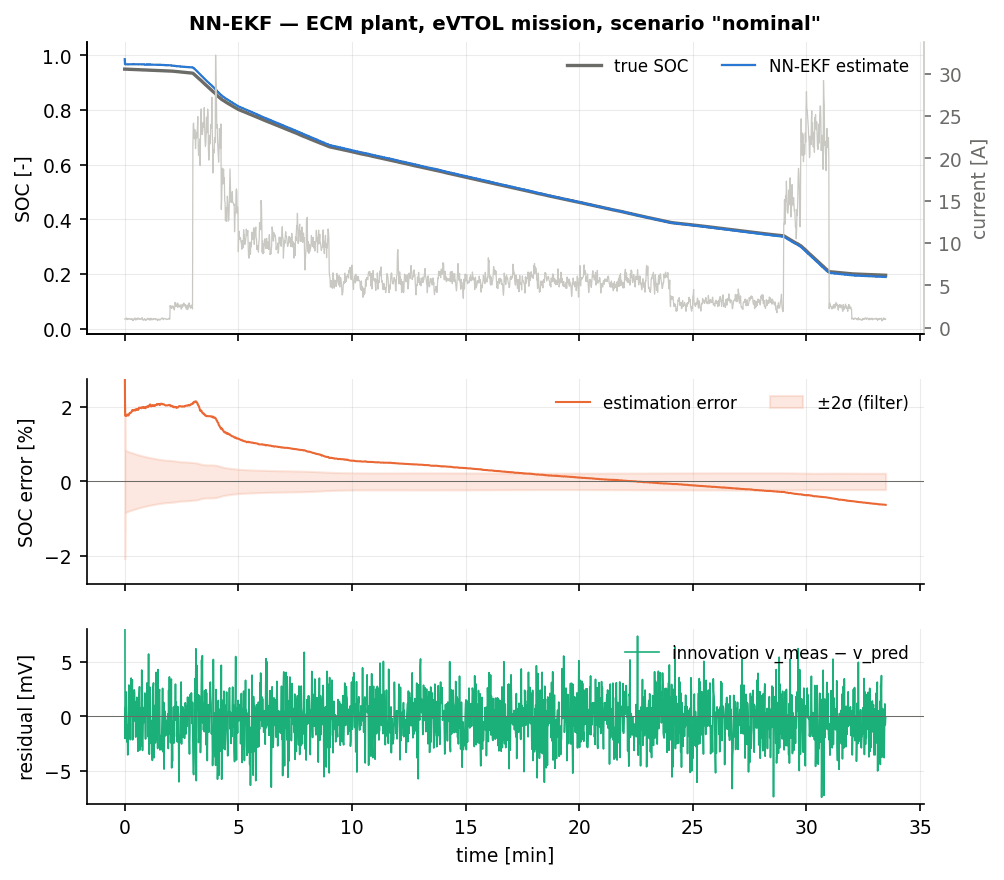
\includegraphics[width=\textwidth]{figures/cell_NNEKF_nominal.png}
\caption{NN-EKF on the nominal eVTOL mission: true and estimated SOC (top), estimation error with
the $\pm2\sigma$ band (middle), voltage residual (bottom).  The residual network is fitted to
Preisach cells; on this plain cell it injects a systematic voltage offset that the filter converts
into a \SI{0.28}{\percent} SOC bias, and the hysteresis-state transient keeps the error above
\SI{2}{\percent} for the first \SI{200}{\second}.}
\end{figure}
\begin{figure}[H]\centering
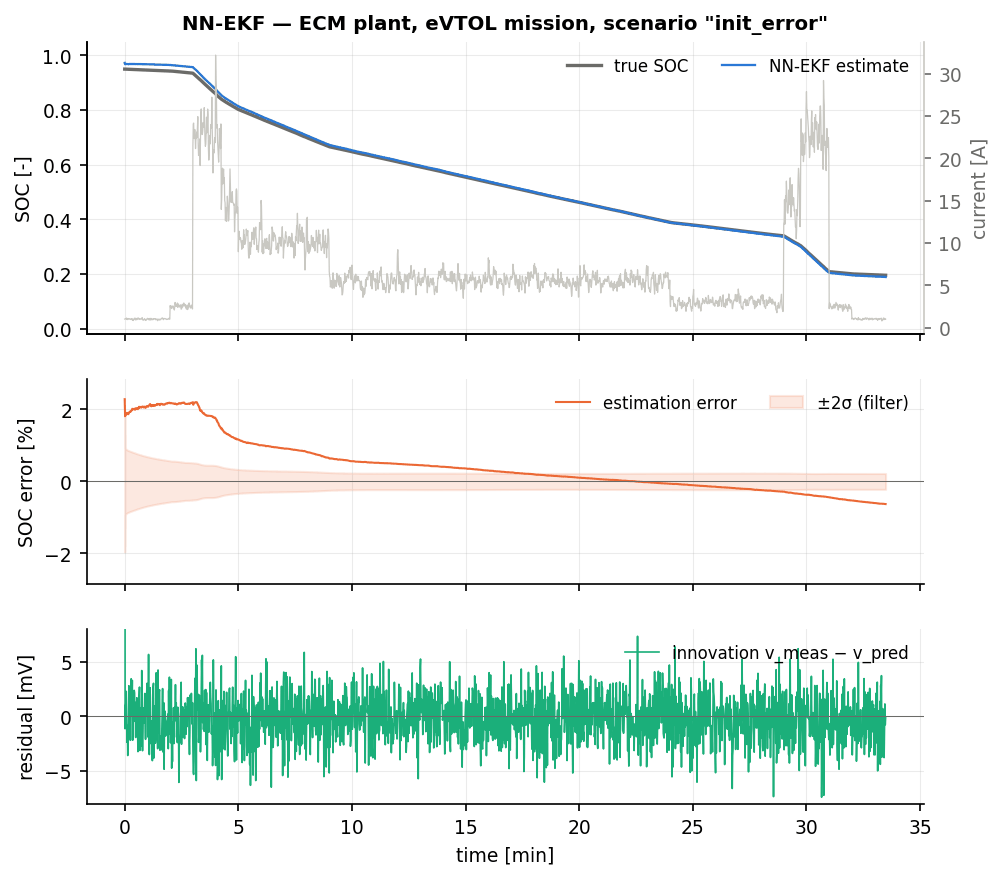
\includegraphics[width=\textwidth]{figures/cell_NNEKF_init_error.png}
\caption{NN-EKF with a \SI{35}{\percent} initial SOC error: the OCV feedback removes the initial
error within the first sample, exactly as for the plain EKF; what remains is the same
hysteresis-state transient as on \texttt{nominal}.}
\end{figure}

All numbers below are three-seed means in per cent SOC from Table~\ref{tab:cell_NNEKF}.

\paragraph{Target scenarios.}  On \texttt{preisach} the hybrid reaches
$\mathrm{rmse}/\mathrm{rmse_{ss}} = 0.24/\SI{0.10}{\percent}$ against the EKF's
$0.58/\SI{0.20}{\percent}$ --- a factor of two in steady state, and \textbf{the best figure of any
estimator in this report on that scenario}: the next best result, shared by a dozen filters
including the plain EKF, is \SI{0.20}{\percent}, so the hybrid is alone at half the field's error.
It is also the scenario with the lowest voltage residual of the whole NN-EKF sweep
($\mathrm{RMSE}_v = \SI{0.77}{\milli\volt}$, against the EKF's \SI{0.81}{\milli\volt}), which is
the direct evidence that the learned term is reproducing a real physical effect rather than
absorbing estimation error.

On \texttt{aged\_cell} the picture is much weaker than in the development runs: $1.52/1.44$ against
the EKF's $1.18/1.52$, i.e.\ a \SI{5}{\percent} improvement in steady state and a \SI{29}{\percent}
\emph{degradation} in full-run RMSE.  The residual model was fitted on cells of nominal capacity
and nominal resistance; a \SI{37.5}{\percent} $R_0$ growth is simply outside what
$r(\soc,i,T)$ was ever shown, and the largest voltage residual of the sweep
($\SI{5.61}{\milli\volt}$) confirms that the augmented output equation is not describing this cell.
The claim that the method helps on aged cells, which the development runs supported, does not
survive the final three-seed run and is withdrawn.

\paragraph{An unexpected win.}  \texttt{param\_mismatch} ($0.95/\SI{0.78}{\percent}$ against the
EKF's $1.28/\SI{1.36}{\percent}$) is now a \SI{43}{\percent} improvement.  Nothing in the method
targets a \SI{30}{\percent} $R_0$ error, and the mechanism is indirect: the learned residual is a
smooth function of $i$ as well as of $\soc$, and the $i$-dependence it absorbed while fitting the
Preisach cells happens to point in the same direction as the missing ohmic drop.  This is luck, not
design --- the ``aged cells in training'' row of the table above shows that a residual model
\emph{deliberately} fitted to an $R_0$ error does much better on this scenario ($0.35$) --- but it
is a reminder that a residual network fitted to one effect does not stay confined to it.

\paragraph{The price.}  On \texttt{nominal} the hybrid gives $0.85/\SI{0.28}{\percent}$ against the
EKF's $0.15/\SI{0.05}{\percent}$: a factor of $5.6$, and entirely systematic.  The truth cell in
\texttt{nominal} has the ordinary one-state hysteresis, the residual model insists on adding the
Preisach correction it was trained on, and the filter --- doing exactly what it should --- converts
the resulting voltage offset into an SOC bias, $\delta z \approx
\delta v/(\partial\ocv/\partial\soc)$.  The same mechanism explains \texttt{hot}
($\SI{0.43}{\percent}$ vs.\ $\SI{0.03}{\percent}$), \texttt{noise\_step} ($0.29$ vs.\ $0.12$) and
\texttt{outliers} ($0.30$ vs.\ $0.21$).  It is an order of magnitude smaller than it was before the
Preisach plant's sign convention was corrected --- the penalty used to be a factor of seventeen ---
but it is still a bias the plain EKF does not have.  Two scenarios escape it: \texttt{cold}
($0.19$ vs.\ $0.16$) and \texttt{sensor\_dropout} ($0.45$ vs.\ $0.46$), where other error sources
dominate.

\paragraph{A transient the table makes visible.}  Five ECM scenarios report
$t_\text{conv} \approx \SI{200}{\second}$ with $|e|_{\max} \approx \SI{3.2}{\percent}$ even though
their steady-state error is \SI{0.3}{\percent}.  The cause is the hysteresis state: the plant is
reset to a fully charged branch, the estimator's $h$ starts at zero, and for the first few minutes
the learned residual --- which assumes the branch --- and the model's own $M h$ term disagree.  The
plain EKF, which has no residual term, converges immediately.  This is a real operational cost:
after every power-up the hybrid needs about three minutes before its estimate is inside
\SI{2}{\percent}, and a system that arms on a fresh SOC reading would have to wait for it or
fall back to the plain filter.

\paragraph{Where the hybrid is still harmful.}  \texttt{combined} ($12.74/\SI{9.58}{\percent}$
against the EKF's $16.02/\SI{12.44}{\percent}$): better than the EKF by \SI{23}{\percent}, but both
are unusable, and both take longer than the flight to converge ($t_\text{conv} = \SI{623}{\second}$
for the hybrid, never for the EKF).  The dominant error there is a current-sensor bias acting on
the \emph{state} equation, which Assumption~\ref{as:nne-dyn} explicitly excludes from the network's
reach; the moving-horizon estimators of Chapters~\ref{ch:mhe} and~\ref{ch:mherti} reach
\SIrange{0.5}{0.7}{\percent} on the same data.

\paragraph{Electrochemical (SPM) plant.}
\begin{figure}[H]\centering
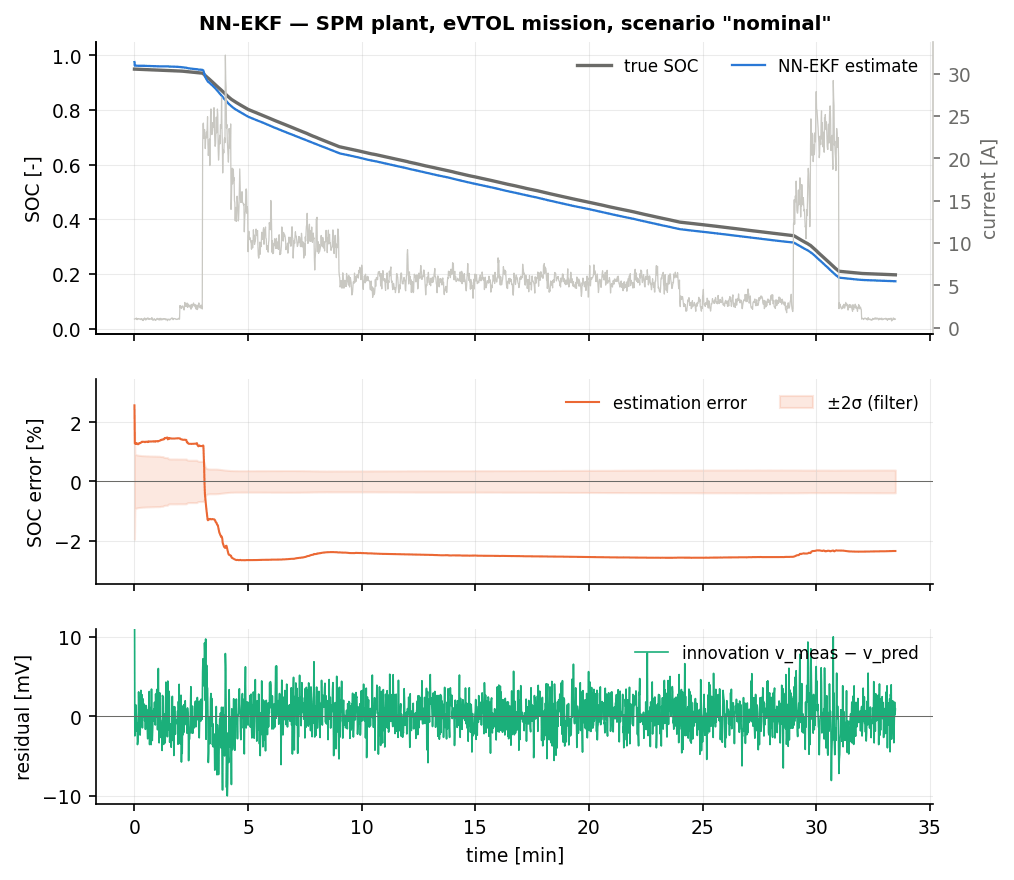
\includegraphics[width=\textwidth]{figures/cellspm_NNEKF_nominal.png}
\caption{NN-EKF on the SPM plant, nominal eVTOL mission.  The residual network was fitted on the
ECM plant and is being applied to a structurally different one; it still beats the plain EKF,
because a bounded learned output term is a cheap way of absorbing a structured voltage residual.}
\end{figure}
Here the hybrid comes into its own, and for a reason that has nothing to do with the population it
was trained on.  The SPM truth plant is an electrochemical single-particle model with
Butler--Volmer kinetics and slow solid diffusion ($\tau_2 = \SI{556}{\second}$); the estimators use
a 2-RC ECM fitted to it, which leaves a \emph{structured} \SI{4}{\milli\volt} residual --- exactly
the kind of object \cref{eq:nne-h} is designed to carry.  NN-EKF gives \SI{2.54}{\percent} on
\texttt{nominal} against the EKF's \SI{3.73}{\percent}, a \SI{32}{\percent} improvement, and it
beats the EKF on seven of the nine SPM scenarios: \texttt{init\_error} $2.50$ vs.\ $3.81$,
\texttt{noise\_step} $2.56$ vs.\ $3.30$, \texttt{current\_bias} $4.87$ vs.\ $5.69$, \texttt{hot}
$1.51$ vs.\ $2.16$, \texttt{sensor\_dropout} $3.16$ vs.\ $5.31$, and most strikingly
\texttt{param\_mismatch} $0.76$ vs.\ $3.13$ --- a factor of four.  The two exceptions are
\texttt{outliers} ($2.46$ vs.\ $1.99$) and \texttt{cold} ($7.61$ vs.\ $7.35$), where the ECM fit is
so far from the SPM plant that a residual model fitted to a different chemistry cannot close the
gap.

The result deserves a caveat, because it is easy to over-read.  The network was \emph{not} trained
on SPM data; what it supplies here is a smooth, bounded, $\soc$- and $i$-dependent correction of
the output equation, and almost any such correction helps when the output equation has a systematic
\SI{4}{\milli\volt} error.  The evidence is that the Fading-EKF, which has no learned component at
all and merely discounts old data, reaches \SI{0.36}{\percent} on the same rows --- seven times
better than NN-EKF.  A fitted residual is worth having when the residual is genuinely a static
function of the state and inputs; when it is better described as ``the model is stale'', a
forgetting factor is the cheaper and stronger tool.

\section{Summary}
NN-EKF keeps the physics and adds one bounded, saturated, $\num{51}$-parameter learned term to the
output equation, exactly as proposed by \citet{charkhgard2010nnekf}.  On the cells the residual was
fitted to it is the best estimator in this report on \texttt{preisach}
(\SI{0.10}{\percent} against a field whose next best is \SI{0.20}{\percent}), it improves
\texttt{param\_mismatch} by \SI{43}{\percent}, and on the electrochemical plant --- whose structured
\SI{4}{\milli\volt} output residual is precisely the object the method models --- it beats the
plain EKF on seven of nine scenarios and by \SI{32}{\percent} on \texttt{nominal}.  It costs twice
the EKF per sample and has a fully specified fallback ($g = 0$) to the plain filter.  Against that:
on a cell from a different population it injects a systematic \SI{0.28}{\percent} SOC bias that no
internal test can detect, it needs about three minutes after power-up before the estimate is inside
\SI{2}{\percent}, its claimed benefit on aged cells did not survive the final three-seed run, and a
plain fading-memory EKF beats it by a factor of seven on the very plant where it looks best.  Use
it when the characterisation campaign and the fleet are the same population and the model error is
genuinely a static function of $(\soc,i,T)$; prefer the online variant of
Chapter~\ref{ch:elmrlsekf} when it is not, and prefer the plain EKF when the lumped model is
already adequate.
